 
\documentclass[A4]{article}

% -- Packages --
\usepackage[utf8]{inputenc}
\usepackage[T1]{fontenc}
\usepackage{fancyhdr}
\usepackage{color}
\usepackage[francais]{babel}
\usepackage{cite}
\usepackage{graphicx}
\graphicspath{{data/}}
\usepackage{listings}
\usepackage{url}
\usepackage{a4}
\usepackage[a4paper, total={5.5in, 9in}]{geometry}
% -- inserer des pdf
\usepackage{pdfpages}
% -- Pour wrapfig = Pour gerer les image + text
\usepackage{wrapfig}
% -- Pour les indentations au 1er paragraph
\usepackage{indentfirst}
% -- Pour quelques truc de math 
\usepackage{amsmath}
\usepackage{SIunits}

% -- For the biblio in the table of content 
\usepackage[nottoc]{tocbibind}

% -- for apendix
\usepackage[toc,page]{appendix}

% -- for the nomenclature
\usepackage{nomencl}
\makenomenclature
\renewcommand{\nomname}{List of Symbols}

% -- Config --
\pagestyle{fancy}

% -- Document --

\title{Implémentation d'un réseau de neurones sur FPGA}
\author{Hugues de Valon\\ Paul Luperini\\ Lucas Mahieu}
\begin{document}

   % -- Page de garde :
\maketitle
   
%\begin{figure}[h!]
%    \centering
%    %\includepdf[pages={1}]{data/FirstPage.pdf}
%    \label{fig:first}
%\end{figure}
   
\pagebreak
\tableofcontents

% -- Sections --
\pagebreak
% Structure file

\section{Introduction}
De nos jours, le chiffrement des données est essentiel pour assurer la sécurité
des transferts de données et préserver la sécurité d'un pays, d'une entreprise
ou la vie privée d'un individu.

L'algorithme AES (Advanced Encryption Standard) est un algorithme très utilisé
en chiffrement des données car reputé incassable. Néanmoins, nous allons voir,
au travers de deux exemples réalisés en travaux pratiques, que cette sécurité
dépend grandement de l'implémentation qu'il en est fait dans un circuit
électronique.\\

Dans un premier temps, nous allons réaliser une attaque par fautes sur un
circuit AES utilisant une protection par redondance d'informations.
Ensuite nous réaliserons une attaque par canaux auxiliaires sur un circuit
AES n'ayant aucune protection spéciale.


\section{TP 1 : attaque par injection de faute}
\subsection{Quelle protections sont mises en place contre les attaques par
fautes ?}


\subsection{Quelles sont les faiblesses de cette sécurité ?}

\subsection{Implémentation de l'attaque par faute}

\subsection{Embarcation du code}


\section{TP 2 : attaque par canaux auxiliaires}
\subsection{Introduction}

Dans cette partie nous allons effectuer une attaque par canaux auxiliaires
sur un chiffrement AES. Cette attaque s'appelle Differential Power Analysis ou
DPA, et consiste à étudier la consommation électrique du système visé sur de
multiples exécutions et d'en déduire par des procédés statistiques l'information
visée, ici la clé de chiffrement.

\subsection{Théorie}
La sécurité d'un système de chiffrement dépend de l'algorithme employé et de
son implémentation sur circuit électronique. Dans le cas de la DPA, nous allons
utiliser des faiblesses d'implémentations pour en déduire la clé de chiffrement
employée.

La SBox (Substitution Box) est le composant non linéaire principal de l'AES. Il
s'agit d'une substitution d'octets, cette opération est effectuée juste après
l'ajout de la clé à la donnée que l'on veut chiffrer. Il est donc possible,
à partir du résultat de la première itération de l'AES qui ne dépendent que
des données d'entrées et de la clé, de retrouver la clé.

La DPA est une attaque par canaux cachés qui utilisent la consommation
électrique du circuit pour valider ou invalider des hyptohèses sur la clé.
La consommation d'un circuit logique dépend grandement des données traitées.
Dans notre cas, il n'y a pas de contre-mesure spécifique utilisée pour
équilibrer la consommation. Ainsi, nous devrions être capables de réaliser
une attaque DPA sur la SBox de l'AES. Néanmoins, nous n'attaquerons pas
la totalité de la clé mais un seul octet, pour des questions de temps de calcul.

\subsection{Travail réalisé}

Tout d'abord, nous devons transformer les fichiers VHDL qui nous ont été donnés
en une description au niveau des transistors, pour pouvoir en extraire une
consommation électrique simulée. Cette étape est réalisée à l'aide de
l'environnement Cadence.

Une fois cette description générée, nous utilisons le simulateur de consommation
électrique Synopsis Nanosim pour obtenir les profils de courants selon certains
stimulis.

\begin{figure}[h!]
    \centering
    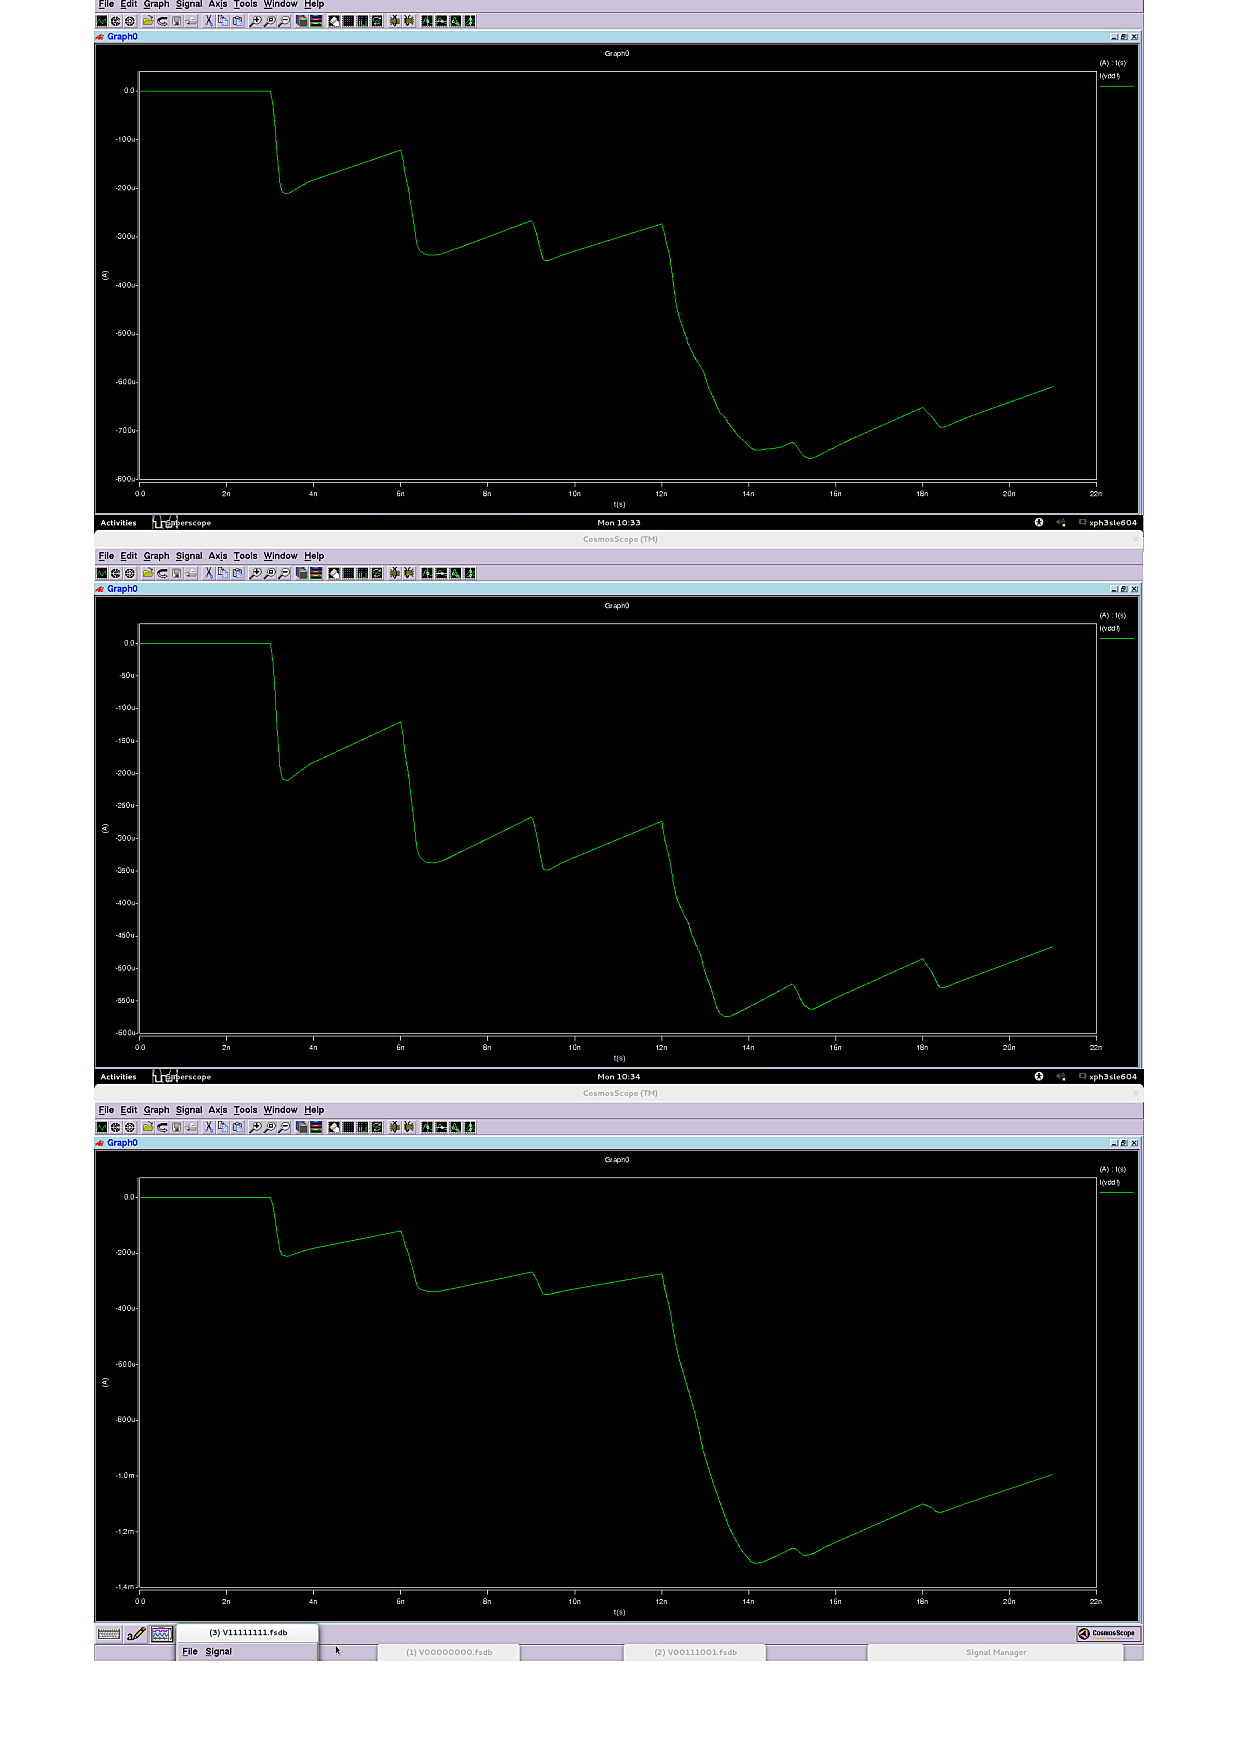
\includegraphics[width=\textwidth]{data/courantsImage}
    \caption{Traces de courants pour différents stimuli}
    \label{fig:courants}
\end{figure}

La figure~\ref{fig:courants}~page~\pageref{fig:courants}
 contient les simulations de courants pour différents stimuli
(la première image pour 0, la deuxième 57 et la dernière 255) pour une certaine
clé de chiffrement AES. On remarque de légères différences, qui seront
exploitées par la DPA.\\

Le logiciel d'analyse DPA fourni nous permet de retrouver les clés utilisées.
Il accepte deux paramètres : l'index du bit attaqué et le chemin vers le
dossier contenant les fichiers de simulation.
L'outil lit un fichier de configuration contenant une liste des vecteurs qui
seront utilisés pour la DPA. Ensuite, les données simulées sont collectées à
partir des fichiers de simulation. Pour chaque hypothèse de clé, il partitionne
les traces de simulation de chaque message selon la valeur du bit attaqué.
Enfin, il évalue les différences entre les moyennes de chaque partition et
sélectionne la valeur la plus haute.


\subsection{Résultats}

Suite à nos expérimentations nous obtenons les résultats suivants visibles
sur la figure~\ref{fig:resultsDPA}~page~\pageref{fig:resultsDPA}.

\begin{figure}[h!]
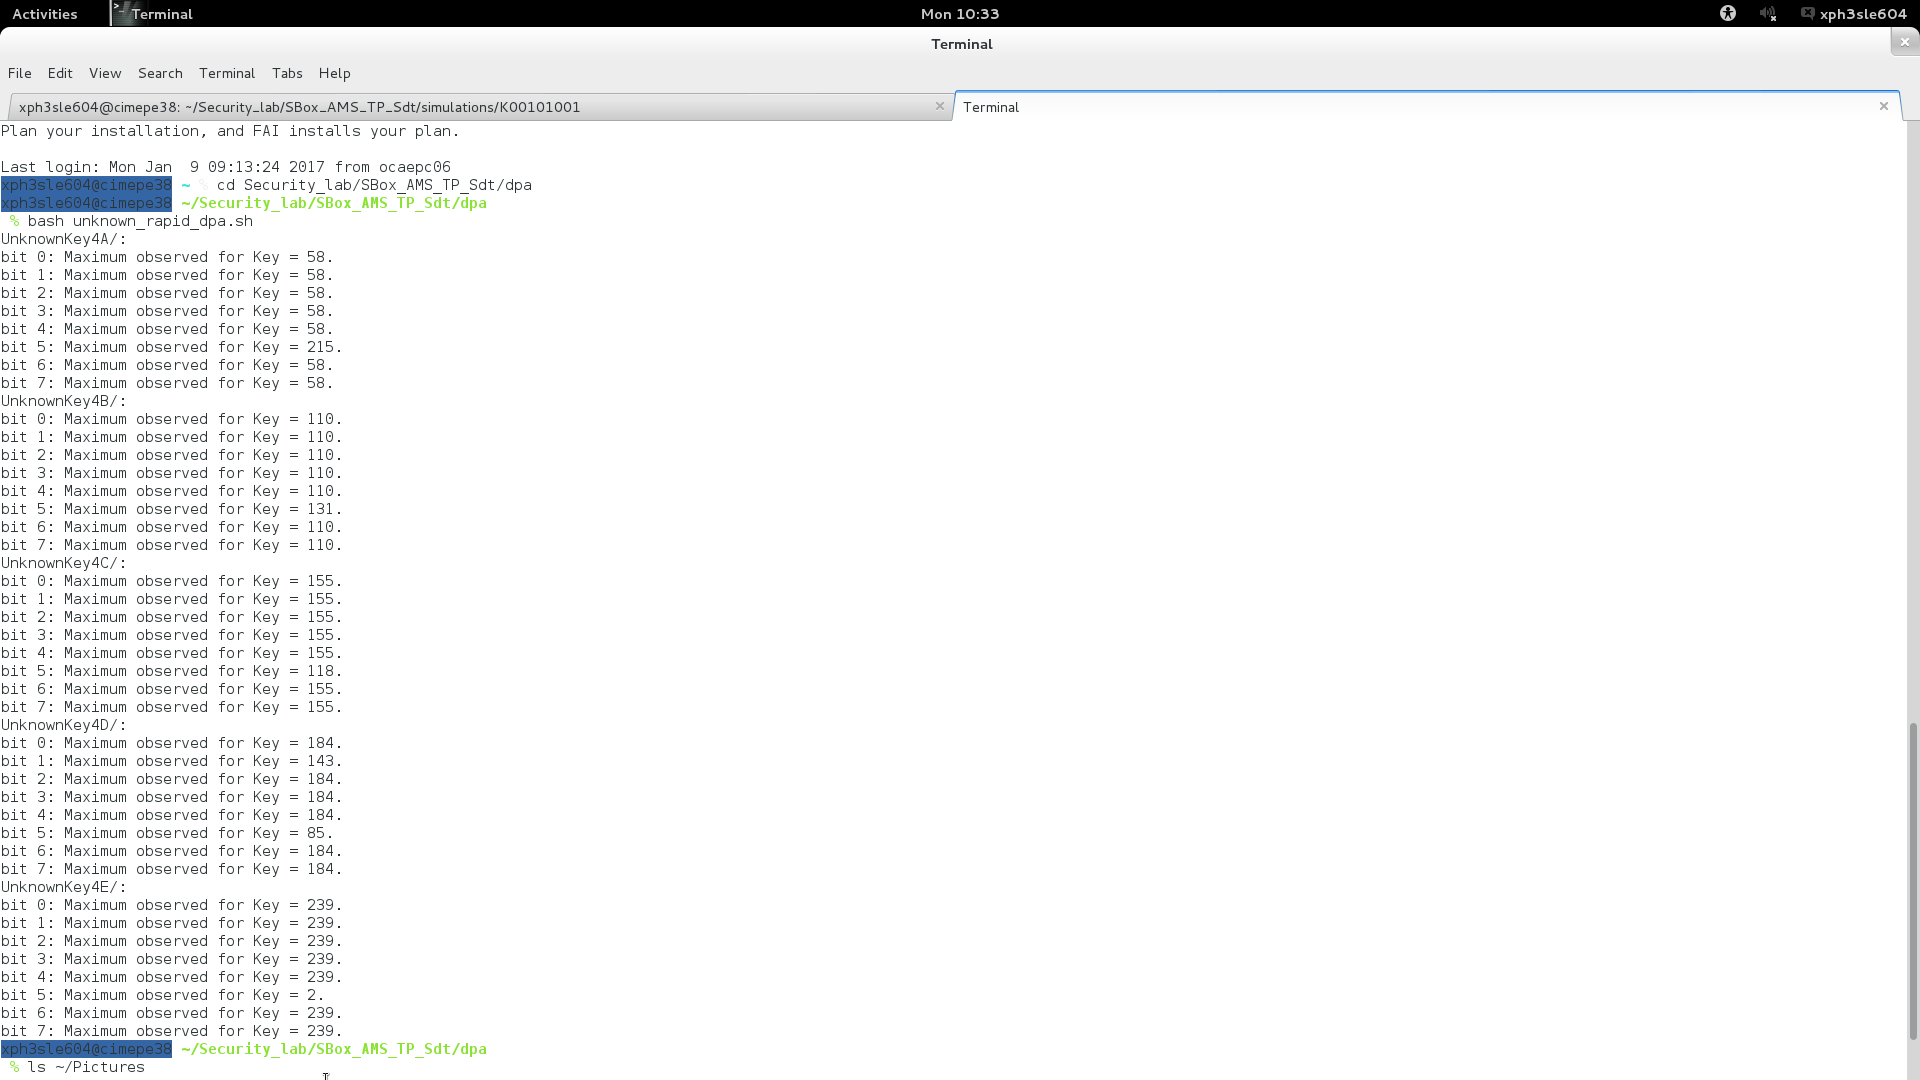
\includegraphics[width=\textwidth]{KeyGroup4}
\caption{Résultats de l'attaque DPA sur l'ensemble de données du groupe 4}
\label{fig:resultsDPA}
\end{figure}

Pour obtenir la clé qui a le plus de chances d'être la clé réelle, il suffit
de prendre celle qui apparait le plus souvent sur les différents lancements
du programme avec des bits différents.

Par exemple dans le cas de la clé 4A, celle qui est apparait le plus souvent est
la 58 (0b111010).

\subsection{Conclusion}

Dans ce TP, nous avons vu comment réaliser une attaque par canaux cachés DPA, et
obtenir la clé de chiffrement. Pour se protéger de telles attaques, il faut
rendre la consommation de de courant insensibles aux données d'entrée afin
d'équilibrer la consommation de courant, et rendre inutile la DPA qui se base
sur les différences. Néanmoins, en pratique cela reste très compliqué, car la
plus légère différence peut être une faiblesse exploitable.


\section{Conclusion générale}
Durant les séances de travaux pratiques, nous avons mis en évidence
deux attaques classiques sur des circuits électroniques implémentant
l'algorithme AES : l'attaque par faute et la DPA.

Cet algorithme, pourtant réputé incassable, devient très vulnérable 
dès qu'il est implementé dans un circuit électronique.
Il est donc essentiel de prendre en compte la sécurité d'un circuit
dès le début de sa conception, et de choisir les bonnes contre-mesures
qui préservent la sécurité du chiffrement tout en ne négligeant pas
les performances.



\end{document}

